\subsection{Разработка структуры клиентской части конструктора}


В данном разделе описываются разработанные структуры клиентской части
конструктора и его диаграммы состояний.

\subsubsection{Структура интерфейса конструктора}

Пользовательский интерфейс конструктора представляет собой
административную панель с набором следующих страниц:

\begin{itemize}
	\item страница аутентификации;
	\item страница регистрации;
	\item страница ботов пользователя конструктора;
	\item страница создания нового бота;
	\item страница запуска бота;
	\item страница редактирования бота.
\end{itemize}


Каждая страница состоит из верхней панели и содержимого страницы.
Верхняя панель содержит ссылки на страницы аутентификации и регистрации,
если пользователь не вошёл в систему, иначе - кнопку “выйти из системы”.
Шаблон представлен на рисунке~\ref{f:general-template}.

\begin{figure}[ht]
	\centering
	\vspace{\toppaddingoffigure}
	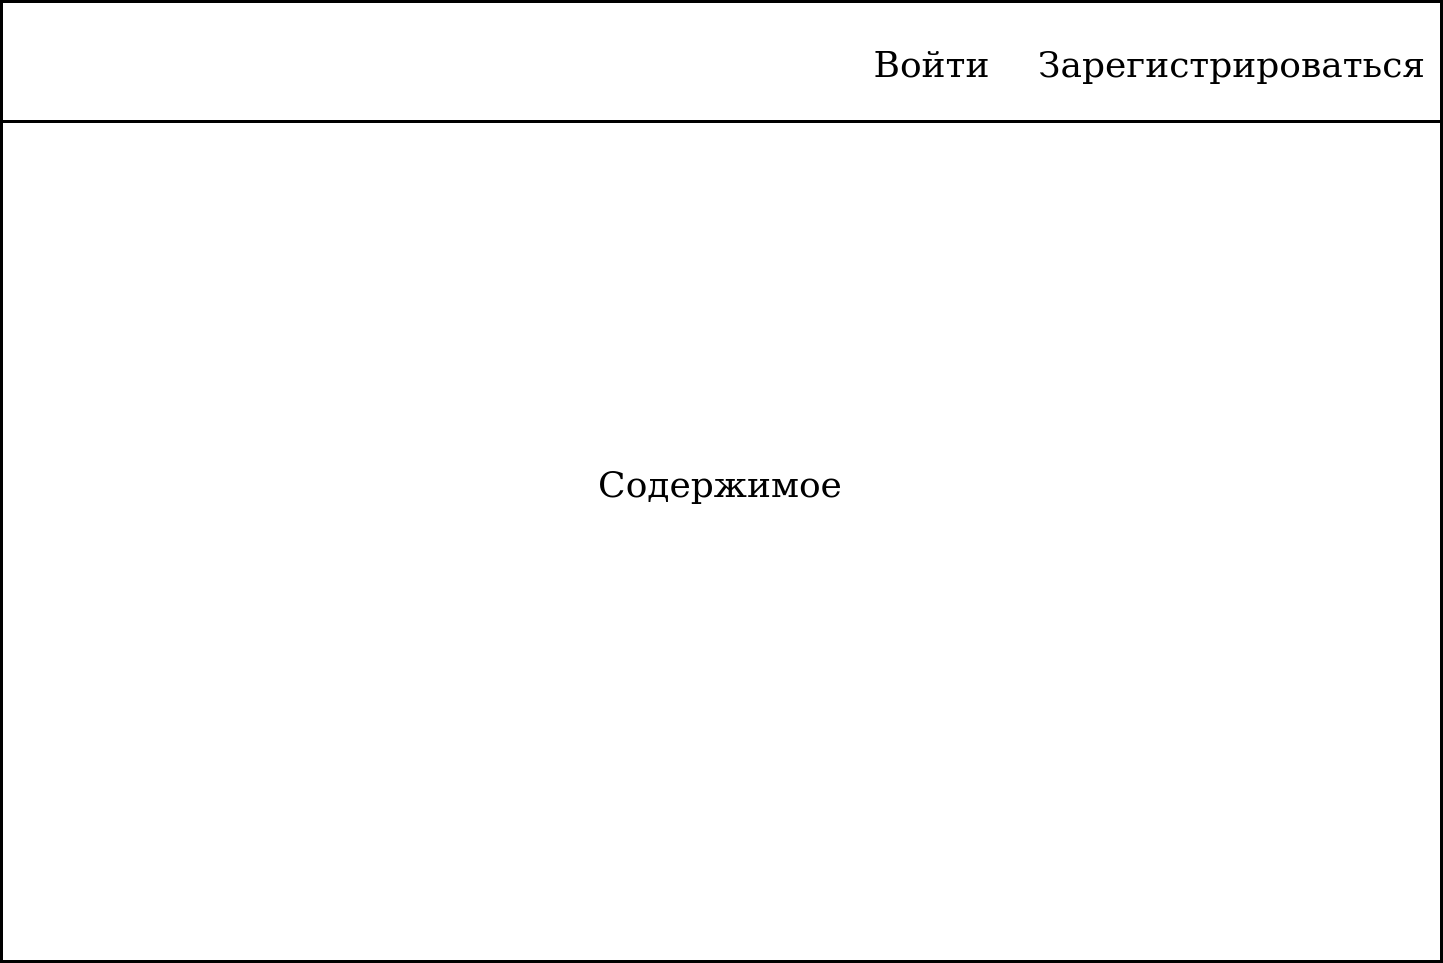
\includegraphics[width=0.6\textwidth]{page-templates/general}
	\caption{Общий шаблон страниц}
	\label{f:general-template}
\end{figure}


Страница аутентификации и регистрации содержат поля ввода логина и
пароля пользователя, под которым располагается кнопка входа или
регистрации. Шаблон содержимого страницы аутентификации представлен на
рисунке~\ref{f:auth-template}.

\begin{figure}[ht]
	\centering
	\vspace{\toppaddingoffigure}
	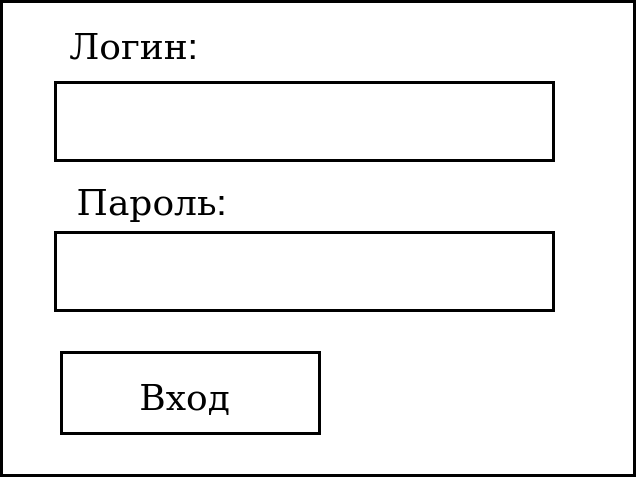
\includegraphics[width=0.4\textwidth]{page-templates/auth}
	\caption{Шаблон содержимого страницы аутентификации}
	\label{f:auth-template}
\end{figure}


Страница ботов содержит список блочных элементов, которые
включают в себя:
\begin{itemize}
	\item название бота;
	\item статус бота;
	\item кнопка для перехода к редактированию бота;
	\item кнопка запуска или остановки бота.
\end{itemize}

Шаблон содержимого страницы списка ботов представлен на
рисунке~\ref{f:list-template}.

\begin{figure}[ht]
	\centering
	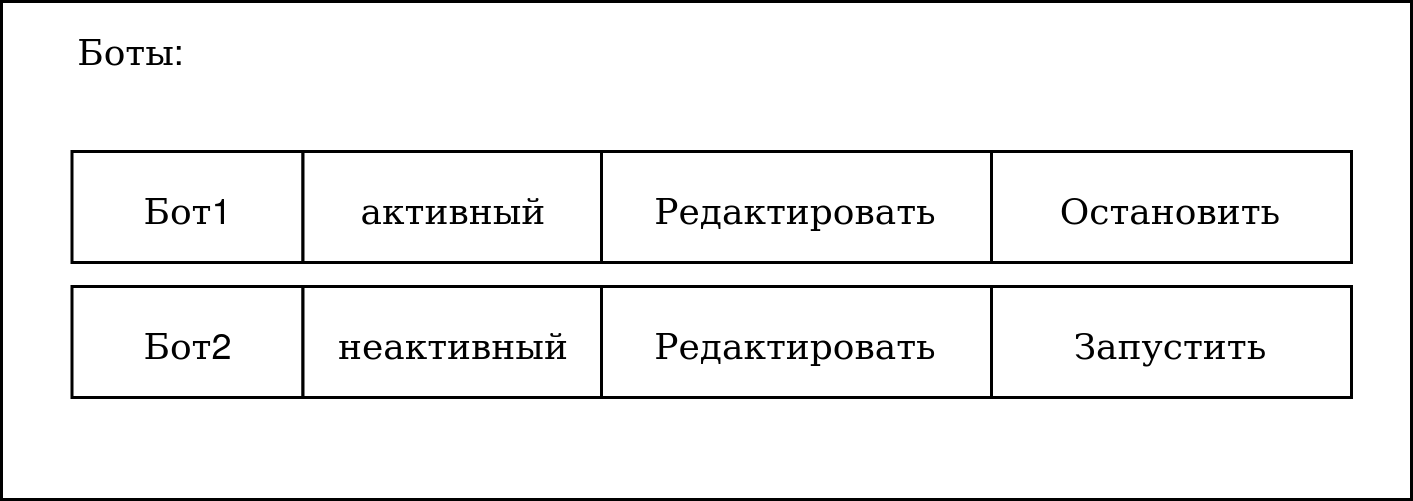
\includegraphics[width=0.7\textwidth]{page-templates/list}
	\caption{Шаблон содержимого страницы списка ботов}
	\label{f:list-template}
\end{figure}

Страница создания бота содержит одно поле ввода, под которым
располагается кнопка создания. Шаблон содержимого представлен на
рисунке~\ref{f:form-template}.


\begin{figure}[ht]
	\centering
	\vspace{\toppaddingoffigure}
	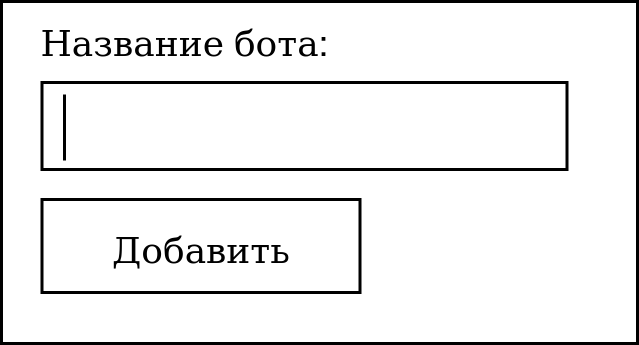
\includegraphics[width=0.4\textwidth]{page-templates/form}
	\caption{Шаблон содержимого страницы создания бота}
	\label{f:form-template}
\end{figure}

Страница запуска бота включает в себя поле ввода токена и кнопку
запуска. Шаблон имеет такую же структуру, как и у содержимого страницы создания бота,
только с другим именованием кнопки и заголовка поля ввода.

Страница редактирования бота содержит визуальный редактор.

\subsubsection{Разработка структуры визуального редактора}

Визуальный редактор ботов представляет собой область, на которой
пользователь может добавлять, редактировать и удалять компоненты, а также
связывать их между собой.

\paragraph{Модульная структура редактора}


Редактор состоит из следующих модулей (Рисунок~\ref{f:mod-client-editor-struct}):

\begin{itemize}
	\item модуль Api-клиента;
	\item модуль контроллера;
	\item модуль представления;
	\item модуль хранилища.
\end{itemize}

\begin{figure}[ht]
	\centering
	\vspace{\toppaddingoffigure}
	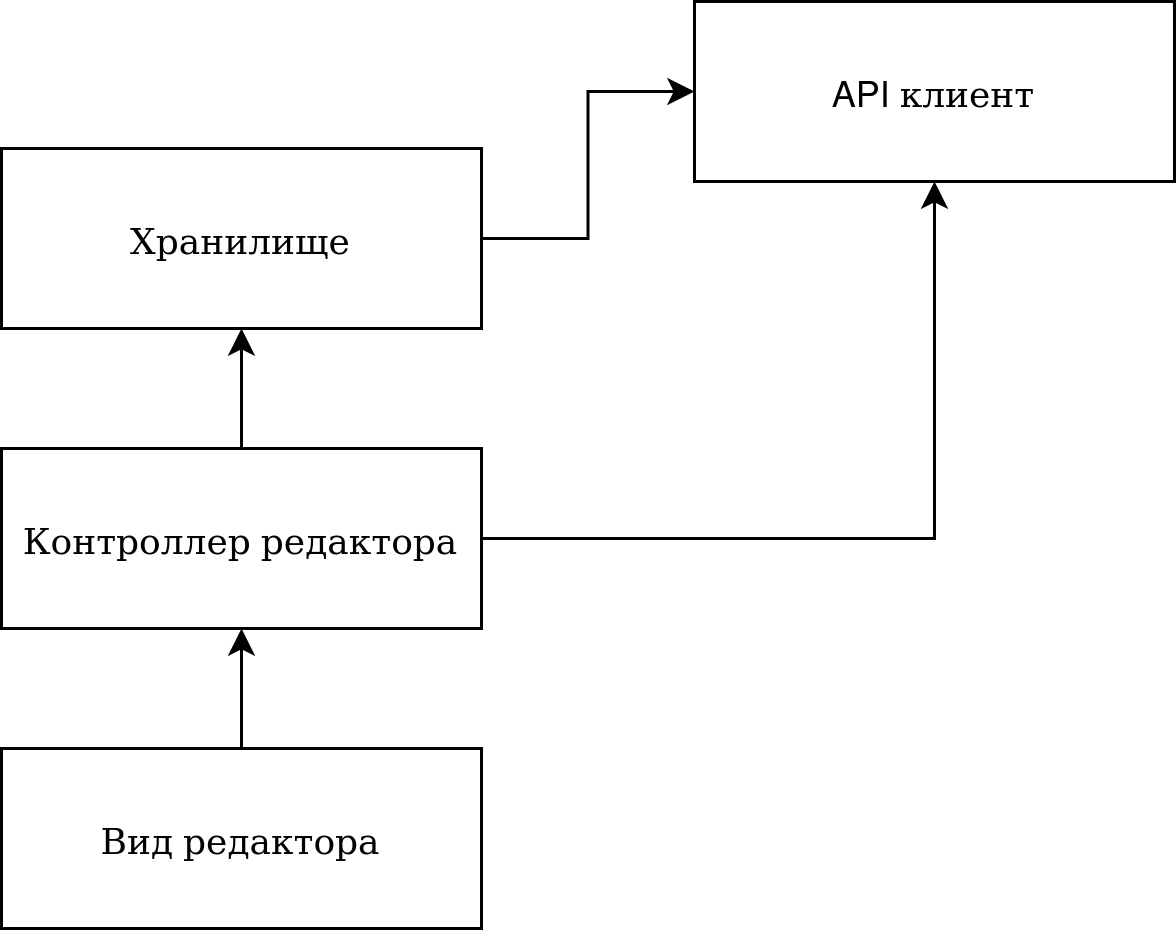
\includegraphics[width=0.7\textwidth]{structures/client-editor/mod}
	\caption{Модульная структура редактора}
	\label{f:mod-client-editor-struct}
\end{figure}


API клиент содержит в себе функции обращения к серверу конструктора
для получения и обновления данных бота.

Хранилище содержит методы для изменения данных редактора. При
изменении данных хранилища происходит обновление их и на сервере через

API клиент.
Контроллер служит посредником между представлением и хранилищем:
он содержит обработчики, которые меняют состояние редактора. Использует
функции API клиента.

Вид редактора (или представление) содержит в себе компоненты
редактора, от которых идут запросы от пользователя. Запросы передаются
контроллеру, который их обрабатывает.


\paragraph{Компонентная структура редактора}

Редактор можно разбить на иерархический набор компонентов: где
вышестоящий компонент является родителем, а компонент, который в нем
содержится, - дочерним.

Компоненты общаются друг с другом посредством передачи параметров
и вызова событий. Родительский компонент вызывает дочерний с помощью
передачи параметров, а также отлавливает события дочернего элемента при
изменении его состояния.

Компонентная структура визуального редактора представлена на
рисунке~\ref{f:comp-client-editor-struct}.

\begin{figure}[ht]
	\centering
	\vspace{\toppaddingoffigure}
	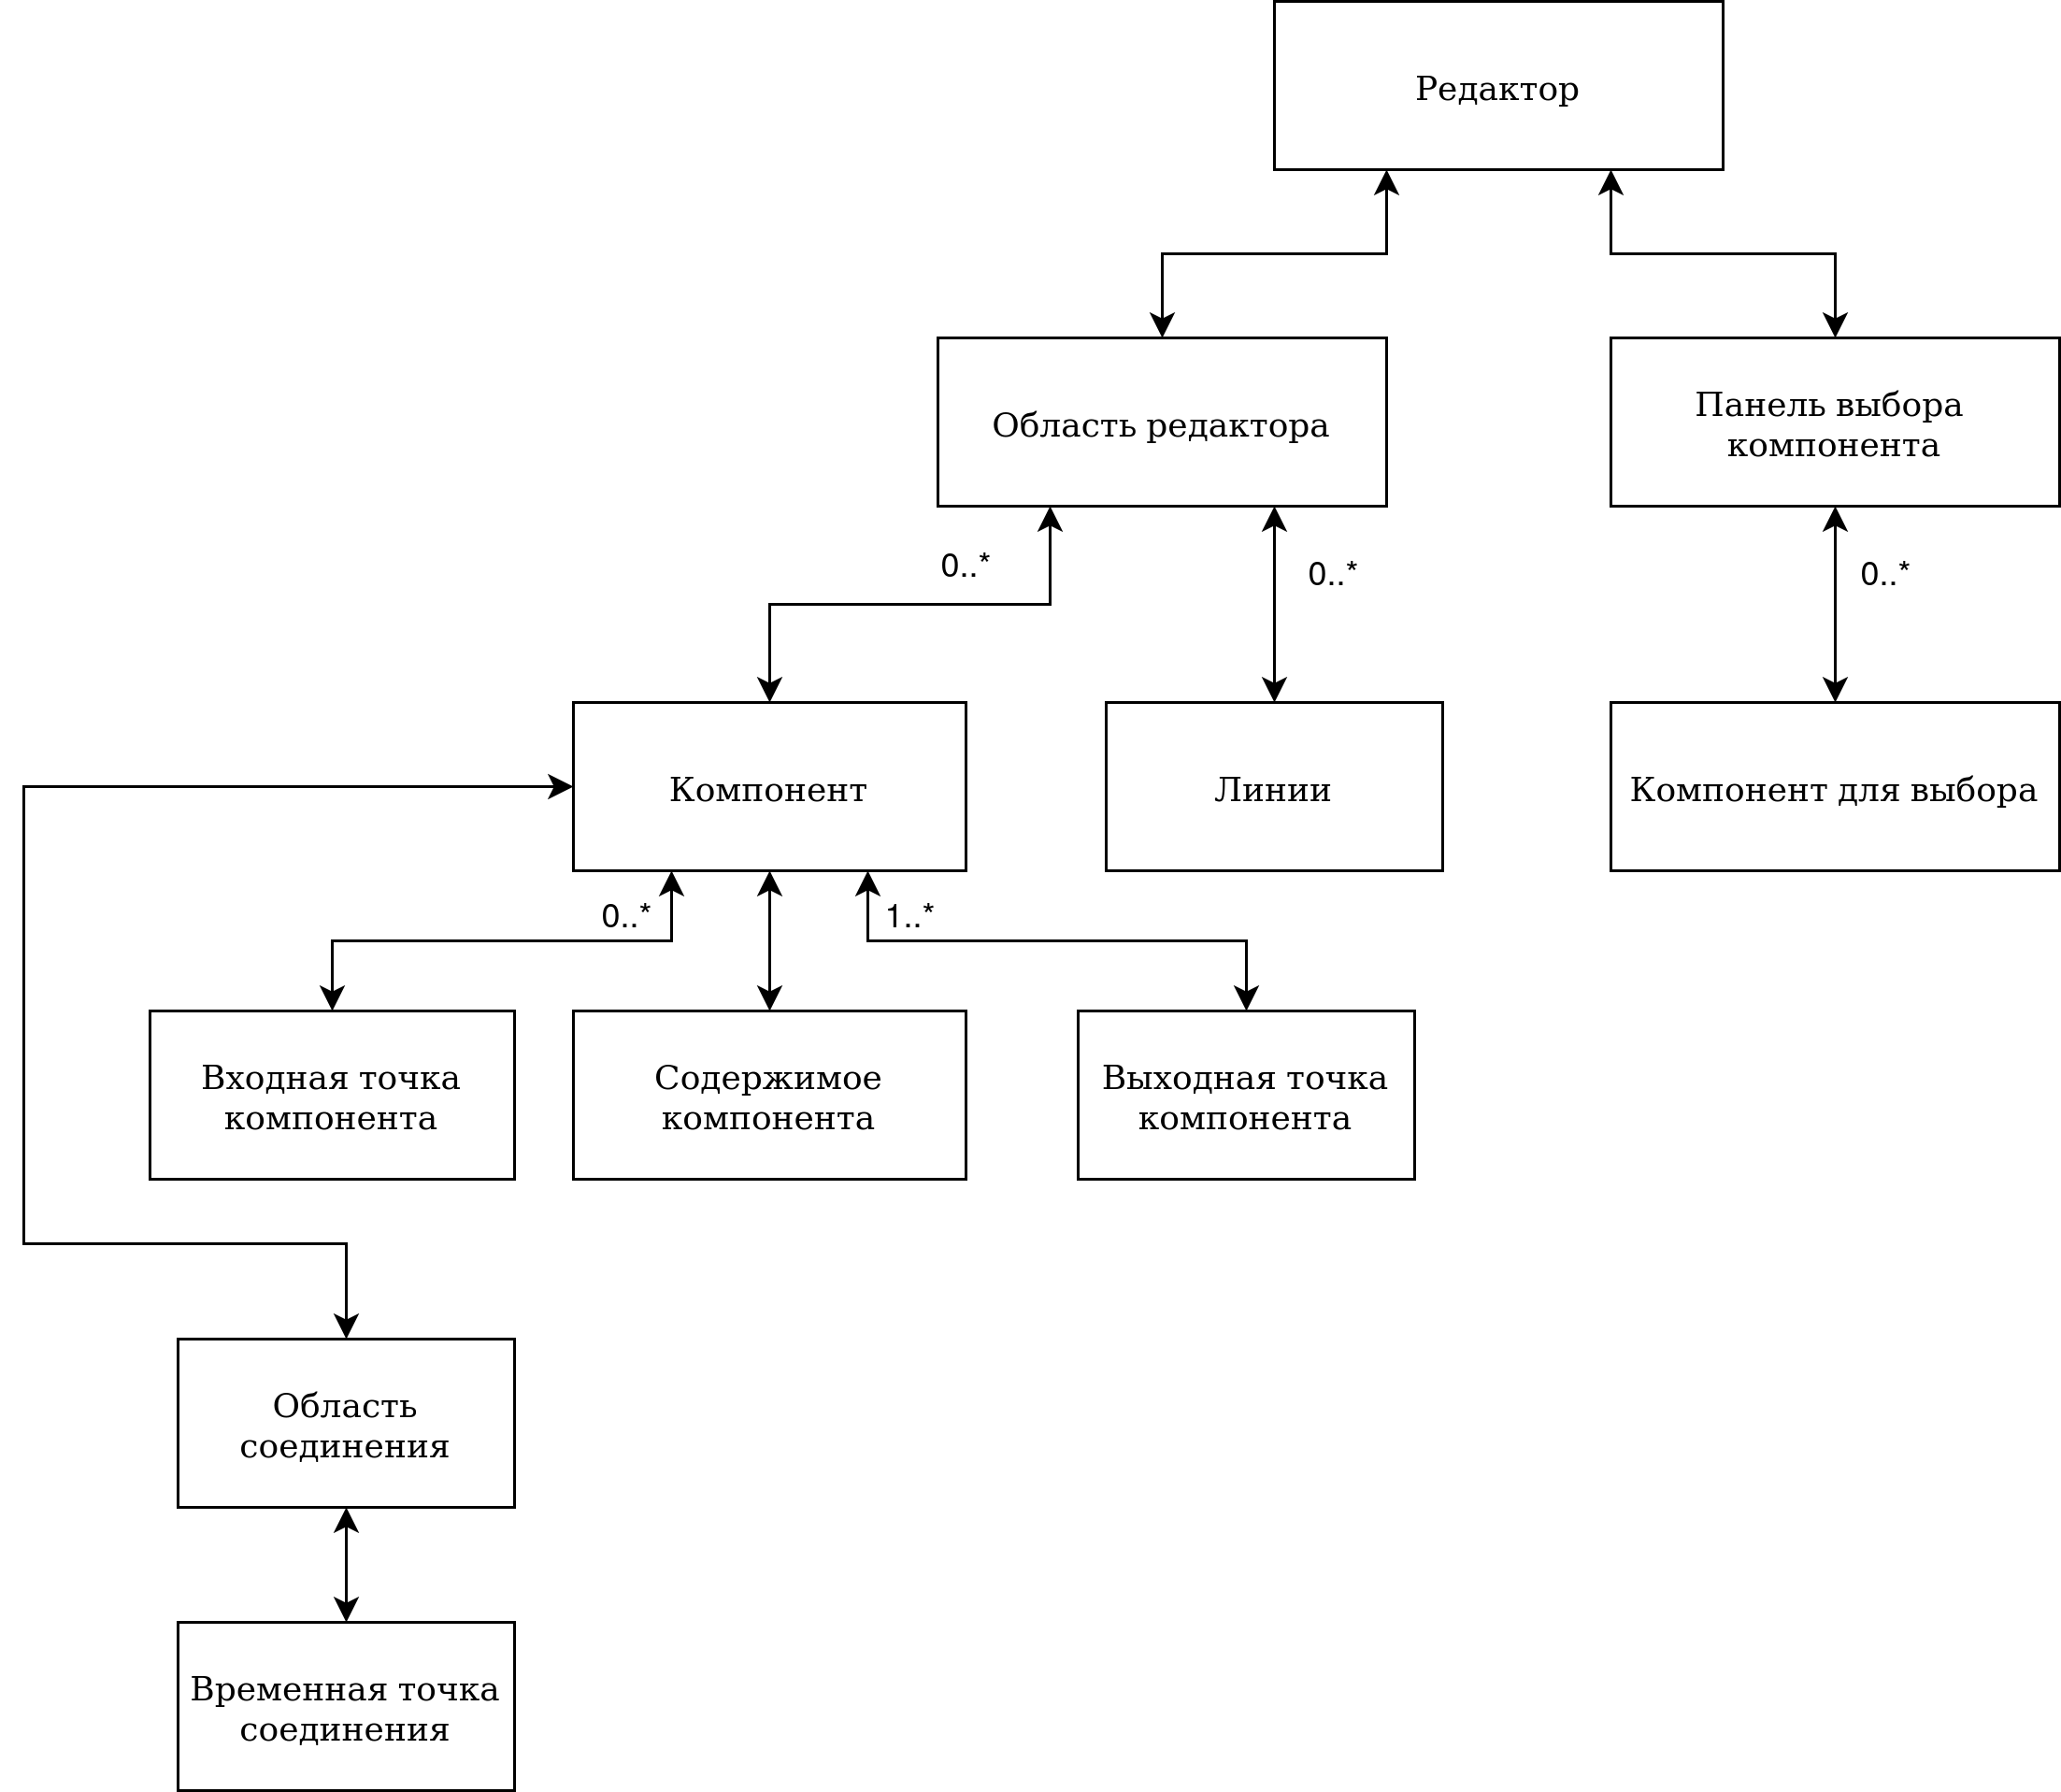
\includegraphics[width=0.9\textwidth]{structures/client-editor/comp}
	\caption{Компонентная структура редактора}
	\label{f:comp-client-editor-struct}
\end{figure}

На самой высокой ступени стоит компонент редактор. Он хранит все
состояние приложения, а также изменяет его с помощью контроллера. Он
состоит из области редактора и панели добавления компонентов.

Панель компонентов содержит разные виды компонентов, которые
можно добавить на область редактора путем перетаскивания.

В области редактора содержится набор компонентов бота и их
соединений.

Компонент бота содержит в себе следующие компоненты:
\begin{itemize}
	\item содержимое компонента;
	\item входные точки компонента;
	\item выходные точки компонента;
	\item область соединения.
\end{itemize}

Компоненты включают в себя разные виды содержимого. Содержимое
зависит от типа компонента.

Чтобы контролировать переход по компонентам присутствуют
элементы соединений – точки соединения. Благодаря им можно располагать
линии между компонентами и тем самым связывать их.

Существует три вида точек соединений:
\begin{itemize}
	\item входная точка;
	\item выходная точка;
	\item временная точка.
\end{itemize}

Входная точка. Служит для обозначения места соединения у
следующего компонента. Может быть несколько – зависит от количества
предыдущих компонентов. При нажатии на данный элемент будет
происходить событие отвязки.

Выходная точка. Служит для указания следующего компонента. Может
быть несколько - зависит от типа компонента. При нажатии на точку будет
происходить событие начала соединения.

Временная точка соединения – элемент, который помогает
пользователю обозначить место соединения у следующего компонента.
Данная точка располагается на области соединения компонента. Вызывает
событие конца соединения при отжатии левой кнопки мыши на этом элементе.
При этом событии происходит скрытие временной и вставка входной точки.

Область соединения компонента представляет собой место, где
возможно расположение входных точек. Область охватывает края
компонента.

Также у каждого компонента присутствует кнопка удаления.

Расположение компонентов на шаблоне визуального редактора
представлено на рисунке~\ref{f:editor-template}.

\begin{figure}[ht]
	\centering
	\vspace{\toppaddingoffigure}
	\includegraphics[width=0.9\textwidth]{page-templates/editor}
	\caption{Шаблон визуального редактора}
	\label{f:editor-template}
\end{figure}

\subsubsection{Разработка диаграмм состояний клиентской части конструктора}

\paragraph{Диаграмма состояний клиентской части}

Клиентская часть конструктора имеет определенный набор состояний.
Эти состояния представляют собой страницы, на которых может находиться пользователь.
Диаграмма состояний клиентской части конструктора представлена на
рисунке~\ref{f:client-state-diagram}.

\begin{figure}[ht]
	\centering
	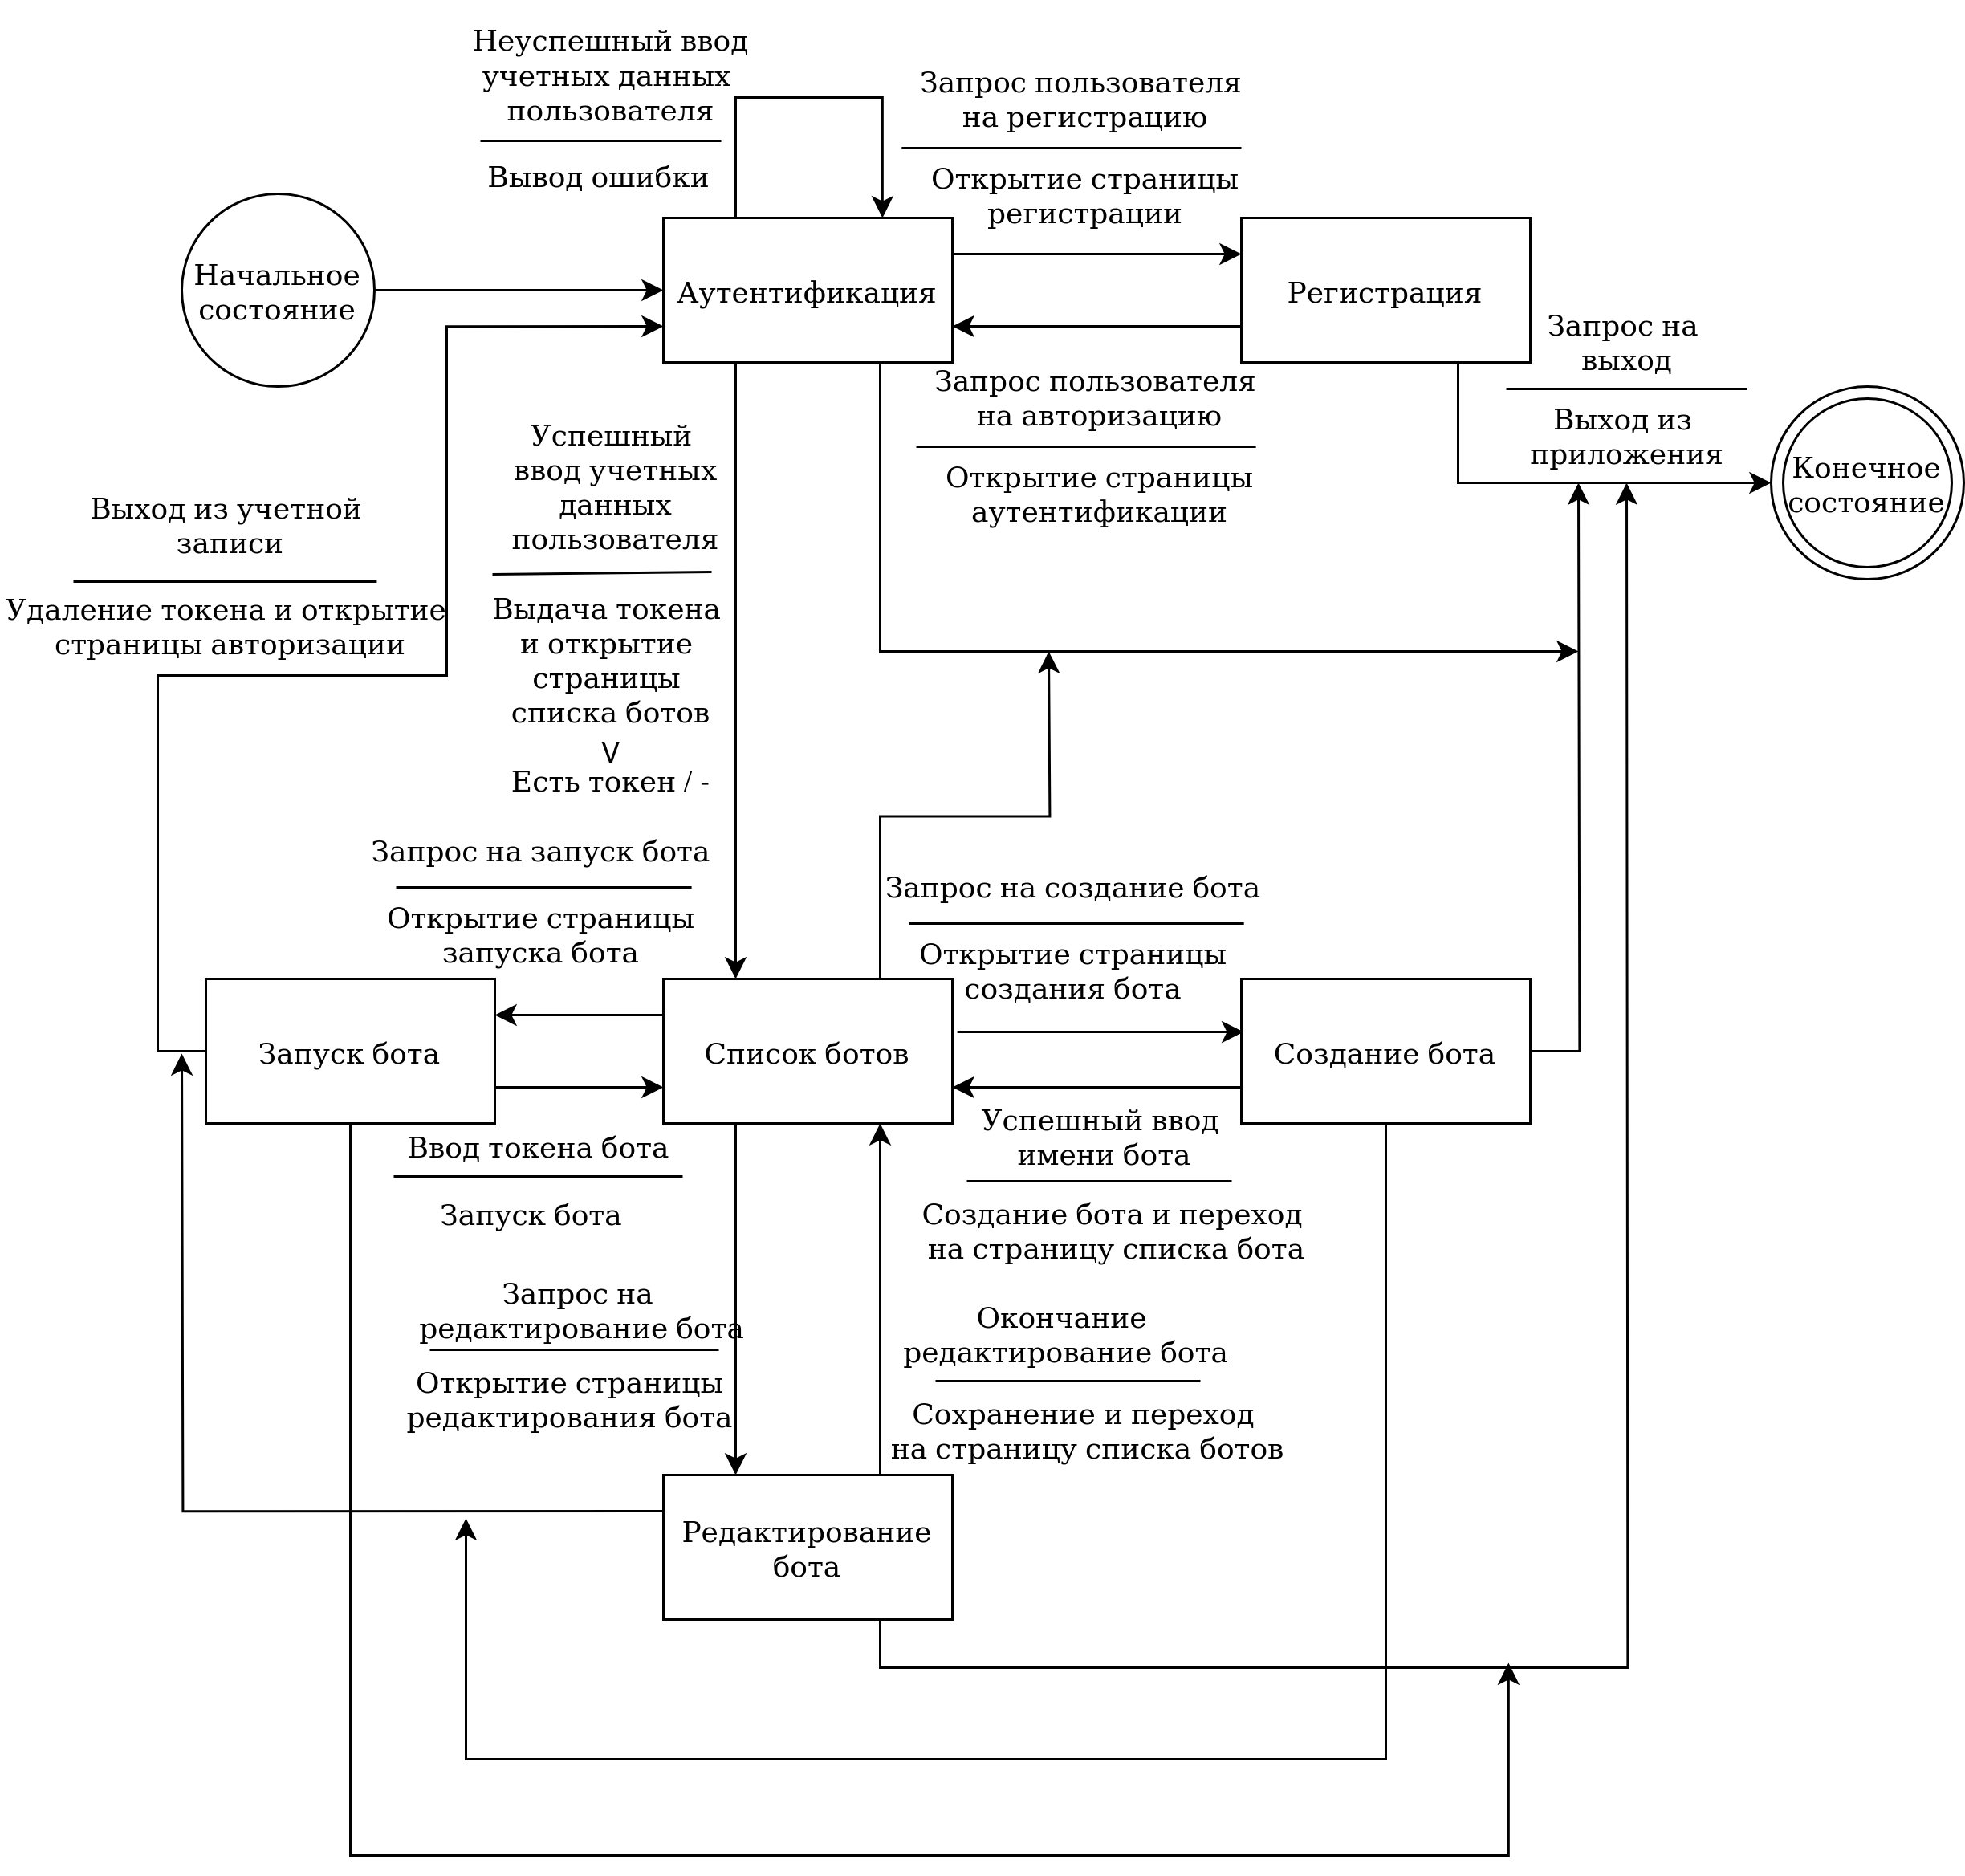
\includegraphics[width=0.9\textwidth]{state-diagrams/client}
	\caption{Диаграмма состояний клиентской части конструктора}
	\label{f:client-state-diagram}
\end{figure}

При запуске приложения пользователя ожидает страница входа в
систему. Если пользователь не зарегистрирован, то ему предлагается перейти
на страницу регистрации.

При правильном вводе логина и пароля пользователю предоставляется
токен доступа, и открывается страница списка ботов, иначе – выводится
ошибка.

На странице списка ботов пользователю предоставляется выбрать бота
для редактирования, удаления или запуска/остановки. Также пользователь
может перейти на страницу создания бота.

На странице создания пользователь может ввести название бота, и после
нажатия на кнопку “создать” происходит создание бота с последующим
возвратом на страницу списка ботов. Список ботов обновляется – в списке уже
присутствует вновь созданный бот.

При запуске бота отрывается страница с вводом токена бота. Если токен
был введен успешно, то происходит запуск бота с возвратом на страницу
списка ботов.

При нажатии на элемент списка ботов происходит открытие редактора,
где пользователь может модифицировать бота: создавать и изменять
компоненты, соединять их.

При закрытии любой страницы происходит выход из приложения, также
при попытке получения доступа к любой из страниц без валидного токена
происходит переход на страницу входа в приложение.

\paragraph{Диаграмма состояний визуального редактора}

Визуальный редактор также имеет конечный набор состояний.
Диаграмма состояний визуального редактора представлена на
рисунке~\ref{f:editor-state-diagram}.

\begin{figure}[ht]
	\centering
	\includegraphics[width=0.8\textwidth]{state-diagrams/editor}
	\caption{Диаграмма состояний визуального редактора}
	\label{f:editor-state-diagram}
\end{figure}


В начале своего запуска визуальный редактор ожидает действия от
пользователя, в зависимости от которых происходит изменение его состояния.

В редакторе присутствует область выбора компонента. Если
пользователь решит выбрать компонент – инициируется переход в состояние
добавления компонента.

В момент перехода в состояние добавления происходит создание
временного компонента, после чего пользователь может его перемещать. Если
конечное расположение компонента выбрано – инициируется переход обратно
в состояние ожидания, при этом временный компонент заменяется
постоянным.

Нажимая на любую выходную точку компонента, пользователь дает
запрос редактору на переход в режим соединения компонентов, следствием
чего является появление линии, которая следует за курсором мыши. Также при
этом у всех других компонентов, кроме начального появляется область
соединения при наведении мыши на неё. При отпускании левой кнопки мыши
на этой области происходит закрепление линии – признак соединения
компонентов. Если же отжатие кнопки мыши происходит вне этой области, то
линия теряется и соединения не происходит. В любом из этих случаев
происходит переход в состояние ожидания.

Отсоединение компонентов происходит при нажатии левой кнопки
мыши на входную точку одного из компонентов, и при этом редактор
переходит в состояние перемещении линии – состояния соединения
компонентов.

При выборе компонента появляется возможность его перемещения.
Если пользователь при уже нажатой левой кнопки мыши на компоненте
начнет её перемещать, то компонент начнёт перемещение за ней – состояние
перемещения. Отпускание левой кнопки мыши закрепит компонент, и
редактор снова начнет ожидать действия от пользователя.

{
\newcommand{\scale}{0.60}

\subsubsection{Расчёт координат объектов визуального редактора}


Область редактора представляет собой координатную плоскость,
на которой располагаются компоненты бота.
Расположение компонента обеспечивается координатами $ ( x_c , y_c ) $,
которые указывают
на левый верхний угол компонента.

При перемещении компонента вычисляются смещения
$ \bigtriangleup x $ и $\bigtriangleup y$
относительно координат нажатой мыши
$ (x_m, y_m) $ по формулам
\begin{gather}
	\bigtriangleup x = x_c - x_m, \\
	\bigtriangleup y = y_c - y_m.
\end{gather}

Данные смещения используются для расчёта новых координат компонента
$ (x_c', y_c') $ при перемещении мыши с координатами
$ (x_m', y_m') $,
которые вычисляются по формулам
\begin{gather}
	x_c' = x_m' - \bigtriangleup x, \\
	y_c' = y_m' - \bigtriangleup y.
\end{gather}

Расположение компонента на координатной плоскости показано
на рисунке~\ref{f:component-crds}.

\begin{figure}[ht]
	\centering
	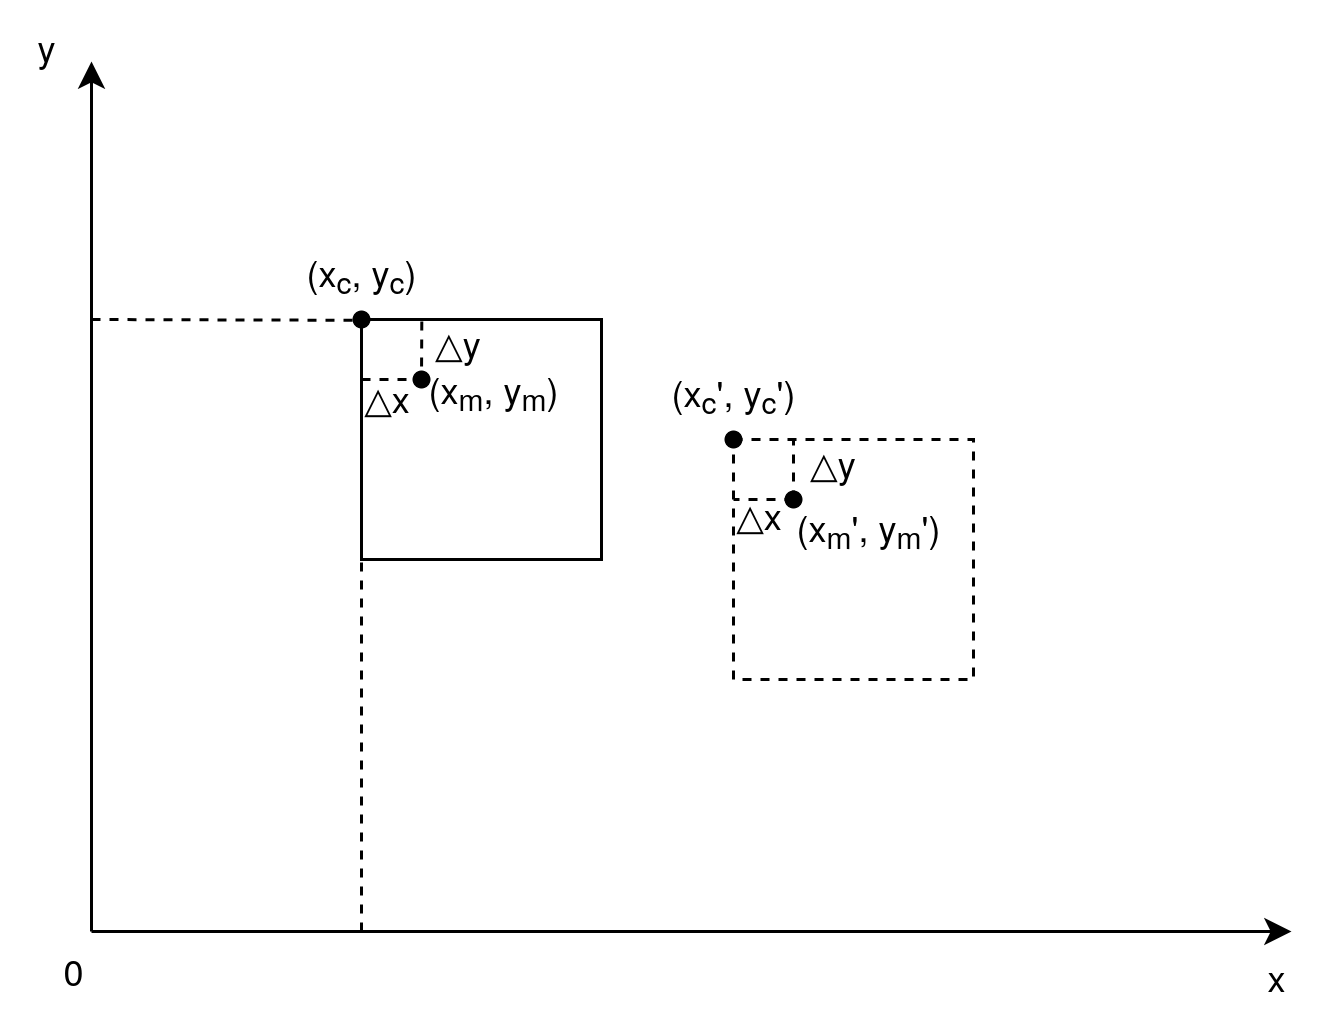
\includegraphics[width=\scale\textwidth]{component-crds}
	\caption{Координаты расположения компонентов}
	\label{f:component-crds}
\end{figure}

Связи между компонентами представляют собой линию со стрелкой.
Линия имеет координаты начала
$ (x_{out}, y_{out}) $
и конца
$ (x_{in}, y_{in}) $, которые представляют собой точки центра окружностей
соединительных точек выхода и входа компонентов.
Расположение связей компонентов на координатной плоскости показано на
рисунке~\ref{f:line-crds}.

\begin{figure}[ht]
	\centering
	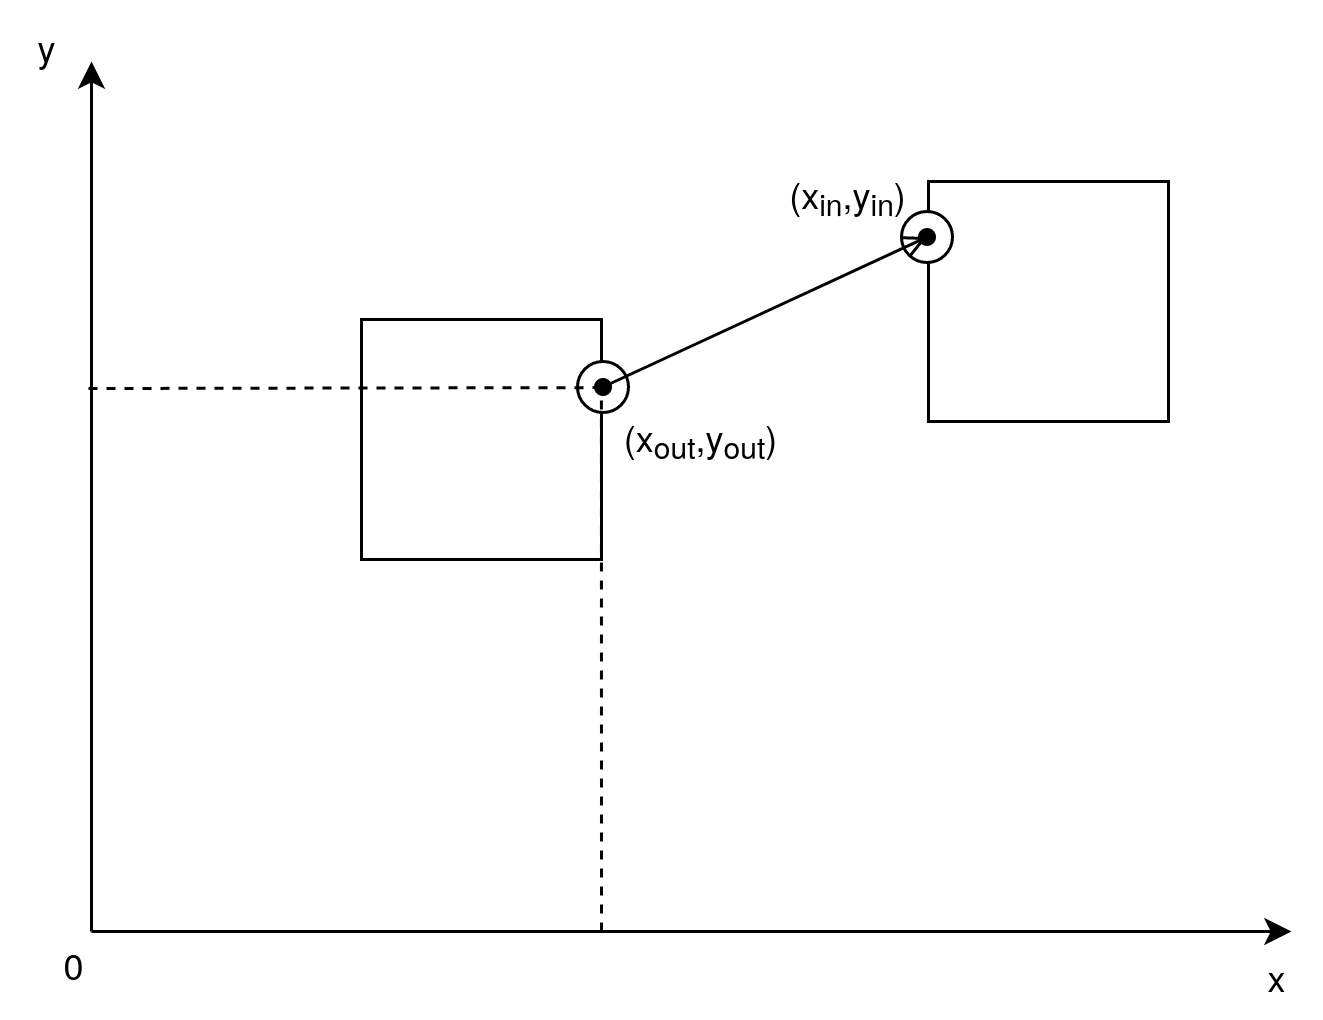
\includegraphics[width=\scale\textwidth]{line-crds}
	\caption{Координаты расположения связей компонентов}
	\label{f:line-crds}
\end{figure}

Стрелка представляет собой две примыкающих к линии прямых.
Стрелка имеет длину
$ a $ и угол между примыкающих прямых $ \alpha $.

Линия между компонентами наклонена под углом $ \beta $ относительно оси $ y $. Угол
вычисляется по формуле
\begin{equation}
	\beta = \arctan(\frac{x_{in} - x_{out}}{y_{in} - y_{out}}).
\end{equation}

Точка
$ (x_a, y_a) $ является окончанием стрелки и её координаты вычисляются по формулам
\begin{gather}
	x_a = x_{in} - sin \beta * a, \\
	y_a = y_{in} - cos \beta * a.
\end{gather}


Расчет смещения $b$ примыкающих прямых относительно основной линии и
смещений $\bigtriangleup x_a$
и $\bigtriangleup y_a$ относительно осей $x$ и $y$ происходит по формулам
\begin{gather}
	b = \tan(\frac{\alpha}{2})*a, \\
	\bigtriangleup x_a = \cos(\beta) * b, \\
	\bigtriangleup y_a = \sin{\beta} * b.
\end{gather}


Сами точки окончания примыкающих прямых
$ (x_{a1}, y_{a1}) $ и $ (x_{a2}, y_{a2}) $
вычисляются по формулам
\begin{gather}
	x_{a1} = x_a + \bigtriangleup x_a, \\
	y_{a1} = y_a - \bigtriangleup y_a, \\
	x_{a2} = x_a - \bigtriangleup x_a, \\
	y_{a2} = y_a + \bigtriangleup y_a.
\end{gather}

Расположение стрелки на координатной плоскости представлено
на рисунке~\ref{f:arrow-crds}.

\begin{figure}[ht]
	\centering
	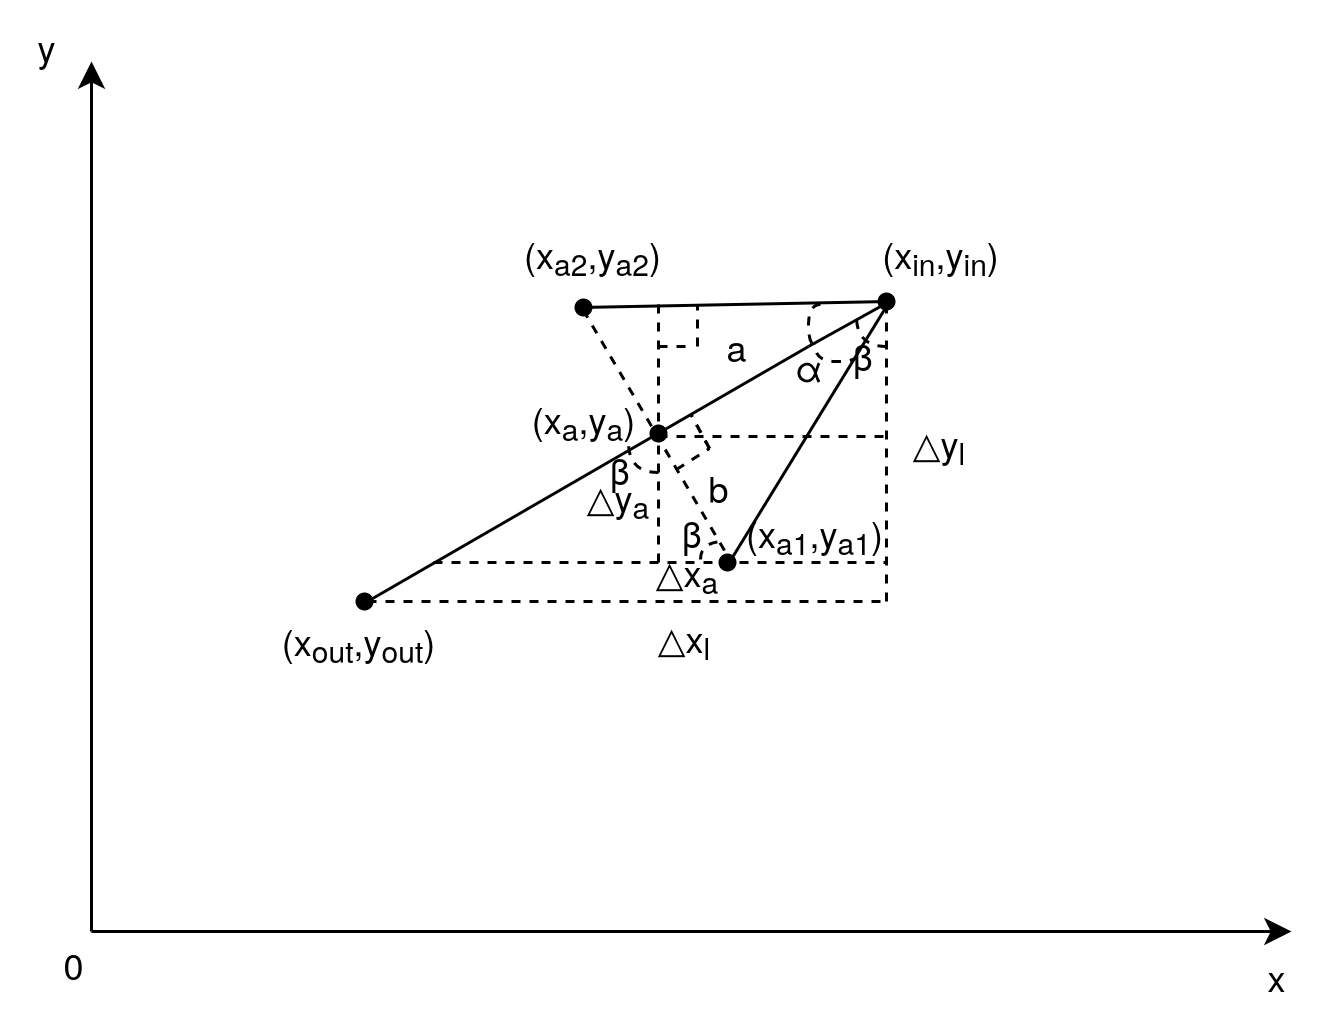
\includegraphics[width=\scale\textwidth]{arrow-crds}
	\caption{Координаты расположения стрелки}
	\label{f:arrow-crds}
\end{figure}


}



